\documentclass[11pt]{article}
\usepackage{amsmath}
\usepackage[sc]{mathpazo} %Like Palatino with extensive math support
\usepackage{fullpage}
\usepackage[authoryear,sectionbib,sort]{natbib}
%\usepackage[square,sort,comma,numbers]{natbib}
\linespread{1.7}
\usepackage[utf8]{inputenc}
\usepackage{lineno}
\usepackage{titlesec}
\usepackage{xcolor}
\usepackage{graphicx}
\usepackage{placeins}
\usepackage{float}
\usepackage{subfigure}
\newcommand{\tom}[2]{{\color{red}{#1}}\footnote{\textit{\color{red}{#2}}}} 
\newcommand{\ali}[2]{{\color{blue}{#1}}\footnote{\textit{\color{blue}{#2}}}}  


\titleformat{\section}[block]{\Large\bfseries\filcenter}{\thesection}{1em}{}
\titleformat{\subsection}[block]{\Large\itshape\filcenter}{\thesubsection}{1em}{}
\titleformat{\subsubsection}[block]{\large\itshape}{\thesubsubsection}{1em}{}
\titleformat{\paragraph}[runin]{\itshape}{\theparagraph}{1em}{}[.]\renewcommand{\refname}{Literature Cited}


%%%%%%%%%%%%%%%%%%%%%
% Line numbering
%%%%%%%%%%%%%%%%%%%%%
%
% Please use line numbering with your initial submission and
% subsequent revisions. After acceptance, please turn line numbering
% off by adding percent signs to the lines %\usepackage{lineno} and
% to %\linenumbers{} and %\modulolinenumbers[3] below.
%
% To avoid line numbering being thrown off around math environments,
% the math environments have to be wrapped using
% \begin{linenomath*} and \end{linenomath*}
%
% (Thanks to Vlastimil Krivan for pointing this out to us!)

\title{An Integral Projection Modeling Approach to Understanding Demographic Effects of Multispecies Mutualisms}


\author{Alexandra Campbell$^{1,\dagger}$ \\ 
	Tom E.X. Miller$^{1,\ast}$}

\date{}

\begin{document}
	
	\maketitle
	
	\noindent{} 1. Program in Ecology and Evolutionary Biology, Department of BioSciences, Rice University, Houston, Texas 77005;
	
	\noindent{} $\dagger$ e-mail: amc49@rice.edu\\
	\noindent{} $\ast$ e-mail: tom.miller@rice.edu
	
	\bigskip
	
	\textit{Keywords}:  Integral Projection Model, \textit{Cylindropuntia imbricata}, population fitness, multi-species mutualism, complementarity, sampling effect, portfolio effect
	
	\bigskip
	
	\textit{Manuscript type}: Article.
	
	\bigskip
	
	\noindent{\footnotesize Prepared using the suggested \LaTeX{} template for \textit{Am.\ Nat.}}
	
\linenumbers{}
\modulolinenumbers[3]

\newpage{}

\section*{Abstract}
\tom{}{I think this is too long for Am Nat requirements. Also, use ``we''.}
Mutualisms are widespread species interactions with diverse and dynamic consequences. 
They are considered more context dependent than other species interactions, meaning there are many different factors which change the outcomes of interactions between mutualists, including partner diversity. 
Partner diversity has become a central focus in the field of mutualisms, expanding previous work from primarily pairwise to multispecies mutualisms. 
It has been shown that pairwise studies are poor predictors of the effects of multispecies mutualistic interactions. 
The diversity of partners in a multi-species mutualism causes varied demographic effects on the population of the focal mutualist which can be explained by several mechanisms: portfolio effect, complementarity, and sampling effect. 

I use the plant-ant multi-species mutualism in which, the cactus \textit{Cylindropuntia imbracata} (tree cholla) pro- duce extrafloral nectar and the ants, \textit{Crematogaster opuntiae}, \textit{Liometopum apiculatum}, \textit{Forelius pruinosus}, and rarer species, provide defense from various herbivores and seed predators. 
I used 18 years of data collected from plant demographic censuses, which includes data such as size, survival, reproductive status, flowers produced, and ant partner for all plants in 8 30$\times$30 m plots at the Sevilleta National Wildlife Refuge in central New Mexico. 
With this data I parameterize a series of Bayesian hierarchical generalized linear vital rate models to determine the impacts of different partners on the focal mutualists. 
I found that different ant partners had different impacts on the vital rates of the tree cholla. 
Specifically, \textit{C. opuntiae} tended plants had advantages in both growth and survival when small, and large \textit{L. apiculatum} tended plants had floral viability advantages. 
With these models I constructed an Integral Projection Model in which I could vary the presence of each partner, creating different “diversity scenarios”, to determine under which diversity scenario the focal mutualist experienced the highest plant fitness, and which mechanism(s) may explain the effects of partner diversity. 
I found that the all scenarios which included the partner \textit{L. apiculatum} resulted in the highest possible fitness for the tree cholla. 
Results further suggest that diversity benefits in this system are driven by sampling effect , meaning \textit{L. apiculatum} ants are the "best`` partner.
I also found that partner diversity benefits the focal mutualist in this system in the form of portfolio effect by buffering the tree cholla from the effects of inter-annual variation. 
This study highlights how partner diversity can increase the overall benefits a focal mutualist receives. 
It also highlights the importance of a mechanistic understanding to explain the benefits of this diversity across systems.

\newpage{}
\section*{Introduction}
Mutualisms are species interactions where all participants receive net benefits, leading to higher individual fitness and increased population growth rates. 
They are among the most widespread species interactions \citep{Bronstein1994,Chamberlain2014,Frederickson2013,Axelrod1981,Leigh2010} but can deteriorate into commensalism or parasitism under conditions that elevate costs or dampen benefits \citep{Rodriguez-Rodriguez2017,Song2020,Mandyam2014,Thrall2007, Bahia2022}.
Mutualisms are considered more context dependent than other species interactions \citep{Chamberlain2014,Frederickson2013}, meaning the magnitude and sign of interaction strength are often determined by environmental conditions and species' identities \cite{Noe1994,Leigh2010}.

Mutualism is defined at the level of a species pair (+/+) but these interactions are embedded within multi-species communities, and growing evidence suggests that pairwise interactions are poor predictors of the net effects of multi-species mutualism \citep{Afkhami2014,Palmer2010,Bascompte2009,Dattilo2014}. 
A focal mutualist may interact with multiple guilds of partner types (e.g., plants that interact with pollinators, seed dispersers, soil microbes, and ant defenders) or with multiple partner species within the same guild (e.g., plants visited by multiple pollinator species). 
Within a mutualist guild, partner species often differ in the amount or type of goods or services they provide, making partner identity an important source of context-dependence in mutualism \citep{Stanton2003}. 
Whether and how partner diversity modifies the demographic effects of mutualistic interactions remain open questions within relevance in applied settings \citep{rogers2014}. 

There are multiple mechanisms by which partner diversity can influence the net benefits accrued by a focal mutualist, mirroring the mechanisms by which, at a larger scale of organization, biodiversity can influence ecosystem function \cite{Yeung2006,Barrett2015,Ushio2020}. 
First, when there is a hierarchy of fitness effects (a consistent ranking of best to worst mutualists), a more diverse sample of the partner community may be more likely to include the best partner \cite{Frederickson2013}.
This can lead to an apparent benefit of diversity driven by a sampling effect \cite{Batstone2018}. 
However, if partner associations are mutually exclusive (a focal mutualist may engage with only one partner at a time), then partner diversity may impose opportunity costs, leading to negative effects of a diverse mutualist assemblage relative to exclusive association with the single best partner \citep{Miller2007}. 
Second, even within a single mutualist guild, the benefits conferred by alternative partner species can vary in type and not just degree \cite{Stachowicz2005,Bronstein2006,Stanton2003}. 
This can lead to a positive effect of partner diversity through complementarity of alternative functions \cite{Batstone2018}. 
Interference or synergies between partners can make their combined effect different than the expected from the sum of complementary functions \cite{Afkhami2014}. 
Third, partner species and \tom{herbivores}{notice that ``herbiviores'' does not fit here, at least not yet. you have not said anything about ants and plants, you are talking very generally. put yourself in the mind of a reader as you write, this will help ensure that ideas appear in an order that can be digested.} can have species-specific responses to environmental variation, either spatially \citep{Ollerton2006} or temporally \citep{Alarcon2008}. 
Multiple partners can therefore act as a 'portfolio' that stabilizes fitness benefits and protection across spatial or temporal heterogeneity, leading to positive effects of partner diversity through the portfolio effect \cite{Batstone2018,Lazaro2022,Horvitz1990}. 

Partner diversity can have different effects depending on whether partners are present all at once or sequentially (partner turnover) \citep{Djieto-Lordon2005, Ness2006, Bruna2014,Barrett2015,Ushio2020,Dattilo2014}. 
Sequential associations are likely when alternative partners engage in interference competition for access to a shared mutualist \cite{Kiers2003,Batstone2018,Tgaard2015,Wulff2008}. 
Turnover can happen at different timescales, from minutes to years \citep{Oliveira1999,Horvitz1986}. 
The frequency of partner turnover can impact the level of benefits received by the focal mutualist, particularly if the benefits continue to accumulate with successive turnover (e.g., when sequential partners provide complementary functions) or if they saturate over time \citep{Sachs2004,Fiala1994}.
Directionality of turnover can also influence effects of partner diversity if partner identity changes consistently across ontogeny of a focal mutualist \citep{Fonseca2003,Noe1994,Dejean2008}.
For example, plant susceptibility to enemies can change across life stages \citep{Boege2005,Barton2010}, so the benefits of defensive mutualism with ants are greatest when more defensive partner species align with more vulnerable life stages \citep{Djieto-Lordon2005,Dejean2008}.

Defensive ant-plant mutualisms -- where plants provide food and/or housing to ants that in turn defend them from enemies -- are widespread interactions that offer valuable model systems for the ecology and evolution of mutualism \citep{Bronstein1998, Bronstein2006}. 
Extrafloral nectar (EFN) bearing plants can serve as dietary resources that promote ant abundance and colony size \citep{Byk2011, Ness2009, Ness2006, Donald2022}.
Presence of defensive ant partners is often linked to reductions in herbivory  \citep{Trager2010, Rudgers2004} and demographic advantages for the plant partner \citep{Baez2016}.
Defensive ant-plant mutualisms are commonly multi-species, where a guild of ant partner species share, and often compete for, a plant mutualist \citep{Bronstein1998, Beattie1985, Trager2010, Agrawal1998}.
Ant partners can vary in their ability to deter herbivores \citep{Bruna2014}, and visitation by low quality ant partners can prevent visitation by higher quality partners, consequently causing a reduction in fitness through missed opportunity costs \citep{Fraser2001, Frederickson2005}.
Susceptibility to herbivory can also vary significantly throughout the life stages of the plant \citep{Boege2005}, suggesting that the order and timing of successive partners is important to the fitness impacts of the combined partner guild \citep{Barton2010, Boege2005, Fonseca2003}.
Herbivore identity and pressure can vary inter-annually \cite{Wetzel2023}, much like mutualist identity and presence, meaning the threat plants face can vary just as much as the protection they receive due to temporal stochasticity. 
Recent studies have begun to investigate how ant partner diversity affects plant fitness \citep{Palmer2010,Afkhami2014,Fiala1994,Gaume1998,Dattilo2014,Ludka2015}
However, little is known about the combined effects of partner identity, directional partner turnover, and temporal stochasticity, particularly because the necessary long-term data are rarely available. 
	
This study examined the consequences of partner diversity in a food-for-protection mutualism between the tree cholla cactus (\textit{Cylindriopuntia imbricata}), a long-lived EFN-bearing plant, and multiple species of ant partners.
Previous studies have shown that herbivory by specialized insect herbivores negatively affects plant fitness \cite{Miller2009}, and ant defense reduces herbivore damage \cite{Miller2007}. 
Tree cholla are tended by two common ant species (\textit{Liometopum apiculatum} and \textit{Crematogaster opuntiae}) and several infrequent species, all of which are ground-nesting. 
These ant species locally co-occur but individual plants are typically tended by only one species that patrols the plant around-the-clock and maintains control of the plant's nectar resources for an entire growing season \citep{Ohm2014, Donald2022}. 
Switches between partner species, or between vacancy and ant occupancy, commonly occur from one growing season to the next \citep{Miller2007}. 
Prior experiments suggested a hierarchy of mutualist quality, with \textit{Liometopum apiculatum} providing strong fitness benefits through anti-herbivore defense and \textit{Crematogaster opuntiae} having net negative fitness effects because herbivore deterrence is outweighed by deterrence of pollinators \citep{Miller2007,Ohm2014}. 
However, those studies did not integrate the demographic effects of ant defense across the plant life cycle, nor did they account for inter-annual fluctuations in the \tom{herbivore populations}{I would be careful here -- unless you are using the herbivore counts I don't think you have data on this.}.

We used a unique long-term data set that allows us to explore mutualistic associations with multiple partner species, longitudinal turnover in partner identity at the individual level, and how the demographic effects of alternative partner species varied across plant size structure and nearly 20 years of inter-annual fluctuations. 
We used this observational data set, contextualized by previous experiments, to ask whether and through which mechanism(s) partner diversity affects the fitness benefits of ant visitation for the focal plant partner. 
Specifically, we asked:
	\begin{enumerate}	
		\item{What are the demographic effects of association with alternative partners and how do these effects fluctuate across years?}
		\item{What are the frequency and direction of partner turnover across the plant life cycle?}	
		\item{What is the net effect of partner diversity on plant fitness, and what mechanism(s) explain(s) this effect?}
	\end{enumerate}
We used a hierarchical Bayesian statistical approach to estimate demographic vital rates for hosts in different states of ant occupancy and to quantify state-dependent partner turnover from the long-term data. 
We then used a stochastic, multi-state integral projection model (IPM) that combines diverse effects on vital rates and pathways of partner turnover to quantify effects of partner diversity on plant fitness. 


\section*{Methods}
\subsection*{Study System}
  
This study was conducted in the Los Pi$\tilde{n}$os mountains, a small mountain chain located on the Sevilleta National Wildlife Refuge, a Long-term Ecological Research site (SEV-LTER) in central New Mexico, USA.
This is an area characterized by steep, rocky slopes, and perennial vegetation including grasses (\textit{Bouteloua eriopoda} and \textit{B. gracilis}), yuccas, cacti, and junipers. 
Tree cholla cacti are common in high Chihuahuan desert habitats, with their native range spanning the southwestern USA \citep{Benson1982}. 
These arborescent plants produce cylindrical segments with large spines. 
In the growing season (May to August in New Mexico), the plants initiate new vegetative segments and flower buds at the ends of existing segments. 
While most plants produce new segments every season, only those which are reproductively mature produce flower buds. 
%Tree cholla generally reach at least 9 years of age before beginning to reproduce \citep{Ohm2014}.
Like other EFN-bearing cacti, tree cholla secrete nectar from specialized glands on young vegetative segments and flower buds \citep{Ness2006,Oliveira1999}. 
Flower buds produce more and higher-quality EFN than vegetative segments, making reproductive cholla valuable mutualist partners. 
Smaller cholla produce little to no EFN, so larger cholla, especially flowering individuals, are generally more highly tended \citep{Miller2014}. 

Tree cholla EFN is harvested by various ant species. 
At SEV-LTER, cholla are visited primarily by two species of ground-nesting ants, \textit{Crematogaster opuntiae} and \textit{Liometopum apiculatum}, as well as other rarer species, including \textit{Forelius pruinosus} and unidentified species of \textit{Aphaenogaster} and \textit{Camponotus}.
\textit{L. apiculatum} are the most frequent visitors with $25\% - 60\%$ of tree cholla tended by these ants, followed by \textit{C. opuntiae} visiting between $5\% - 20\%$ of cacti depending on the year \citep{Donald2022}. 
Between $ 30\% 80\%$ of cacti remain vacant in any given year. 
These ants rarely co-occur on a plant, likely due to interspecific competition \citep{Miller2007}: staged introductions of \textit{C. opuntiae} to \textit{L. apiculatum}-tended plants, and vice versa, provoke aggressive responses by resident ants (A. Cambpell, \textit{personal observation}).
Each cholla is visited by a single ant species for the duration of a season, and the species of the visitors can change from one season to the next. 
In late August, the tree cholla stop producing EFN and the ants vacate until the next growing season. 

There are a variety of insect herbivores and seed predators which specialize on tree cholla \citep{Mann1969}. 
A weevil of the genus \textit{Gerstaekeria} feeds on vegetative and reproductive structures and implants their larvae within the plant tissue for the winter. 
A cactus bug, \textit{Narnia pallidicornis}, (Hemiptera: Coreidae) feeds on all cholla parts with a preference for the reproductive structures \citep{Miller2006}.
A seed predator, \textit{Cahela ponderosella}, (Lepidoptera: Pyralidae) attacks developing fruits pre-dispersal and oviposits in open flowers mid-growing season where larvae burrow into the ripening ovary. 
These predators can have significant negative impacts on plant fitness of and depress population growth \citep{Miller2009}.
There is experimental evidence that tree cholla tended by \textit{L. apiculatum} and \textit{C. opuntiae} experience less herbivory than plants from which ants were excluded \citep{Miller2007}. 

\subsection*{Data Collection}
This study is based a long-term demographic data set spanning 2004 to 2023 at SEV-LTER. 
From 2004 to 2008, we censused 134 plants distributed across three spatial blocks. 
This initial census group was discontinued in 2009, when we established six 30 $\times$ 30-meter plots and tagged all tree cholla within those plots. 
Two additional 30 $\times$ 30-meter plots were added in 2011, and this group of eight plots has since been censused annually through 2023 (with the exception of 2020 due to the covid shutdown). 
For all plants, in May or early June of each year we recorded plant survival since the last survey and, for survivors, we recorded the height (cm), maximum crown width (cm), and crown width perpendicular to the maximum (cm).
Size measurements were used to calculate plant volume ($cm^3$) based on the volume of an elliptical cone. 
We recorded reproductive effort as counts of viable and aborted flowerbuds. 
We recorded the ant species present (or vacancy if no ants present).
Occurrences of more than one ant species on one plant were rare (\tom{}{quantify}), and for the purpose of this analysis we classified the plant as being occupied by the more abundant species. 
Plots were searched for new recruits each year, and these were added to the census.
\tom{In total, the data set included \# unique individuals and \# plant-year observations. }{update numbers}
These data were used to fit vital rate models (survival, growth, reproduction) as functions of plant size and ant occupancy state. 

We used additional, smaller data sets from previously published studies to estimate seed and seed bank parameters. 
Ohm et al. \citep{Ohm2014} provide data on the number of seeds per fruit for plants tended by \textit{L. apiculatum}, \textit{C. opuntiae}, or no ants (experimental exclusion). 
Miller et al. \citep{Miller2009} provide data on seed entry to the seed bank and seedling germination and survival rates. 


\subsection*{Multi-state Integral Projection Model}
Integral Projection Models describe population dynamics in discrete time, with functions that relate vital rates to continuous state variables. 
While IPMs are a natural choice for populations with continuous size structure, they can also be modified to accommodate a combination of continuous and discrete state variables, as we do here. 
We constructed a multi-state IPM that stitches together population structure associated with plant size and ant state, allowing us to determine the individual fitness effects of each ant species and the composite effects of multiple partners, with their transition dynamics modeled explictly. 

Given the low frequency of ant species other than \textit{L. apiculatum} and \textit{C. opuntiae} (\tom{}{Quantify this.}) we combined observations of all other ants into an ``other'' category, such that our models included four possible ant states: vacant, \textit{L. apiculatum}, \textit{C. opuntiae}, and ``other''. 
\tom{The ``other'' category was made of unidentified ant species and ant species which occurred at relatively low frequencies compared to \textit{C. opuntiae} and \textit{L. apiculatum} (such as unknown species belonging to the genus \textit{Aphenogaster} and unknown species belonging to the genus \textit{Camponotus}).}{I think you can do better than this because we actually have the designated species in the data. I would report here the actual breakdown (percentages) of species in the ``other'' group. I expect Forelious will be a big chunk of it.}
Ant state is included as a predictor variable in sub-models where there are biologically realistic pathways through which ants could impact the outcome of that process. 
For example, ant partners defend cacti from herbivores, and prior experimental work indicates that ant tending can reduce vegetative tissue loss and floral abortion.
Therefore, ant state was included in sub-models for survival, growth, and flowerbud viability. 
In contrast, we have no reason to expect that ant tending can directly influence the probability of flowering and flowerbud production, independently of its influence on plant size. 
Therefore, these sub-models included plant size but not ant state as predictor variables. 

Following previous studies, we modeled the tree cholla life cycle using continuously size-structured plants where $n(x,a)_{t}$ gives the number of plants of size $x$ and ant state $a$ in year $t$, plus two discrete seed banks ($B^1_{t}$ and $B^2_{t}$) corresponding to 1 and 2-year old seeds. 
Seed bank dynamics are given by:

\begin{linenomath*}
	$$
	B^1_{t+1} = \delta \sum_{a=1}^{A} \int_L^U  \kappa(a') P(x';\pmb{\tau^P}) F(x';\pmb{\tau^F}) V(a;\pmb{\tau^V_{a}}) n(x,a)_{t} dx \\
	$$
	$$
	B^2_{t+1} =  (1 - \gamma_1)B^1_{t}\\
	$$
\end{linenomath*}

\noindent Functions \tom{$P(x';\pmb{\tau^P})$ and $F(x';\pmb{\tau^F})$}{These should be $x$ not $x'$ because we modeled flowering and fertility in year t based on size in year t.} give the probability of flowering and the number of flowerbuds produced, respectively, by plants of size $x'$ in year $t$. 
The proportion of flowerbuds that remain viable through fruit set ($V(a;\pmb{\tau^V_{a}})$) and the number of seeds per fruit (\tom{$\kappa(a')$}{Why is this $a'$? I think it should be $a$. More generally, I think you need to explain your use of primes and how readers should interpret them at the start of model exposition.}) are dependent on ant state $a$ but not size. 
The vector $\pmb{\tau}$ gives year-specific deviates (with mean zero) and appears in functions for which we can estimate temporal stochasticity from the long-term data; superscripts indicate the corresponding vital rate and subscripts indicate that \tom{deviates are specific to plants in ant state $a$}{Why does the tau vector for viability have the $a$ subscript but the others do not?}. 
Seed production is integrated over the size distribution, from the lower $L$ to upper $U$ size limits, and summed over all possible ant states ($A$) giving total seed production. 
Seeds are multiplied by the probability of seed dispersal and survival ($\delta$) to give the number of seeds that enter the one-year old seed bank. 
Plants can recruit out of the year-one seed bank with probability $\gamma_1$ or transition to the two-year seed bank with a probability of $1 - \gamma_1$. 
Seeds in the two-year seed bank are assumed to either germinate with probability $\gamma_2$ or die. 

For the above-ground part of the life cycle, the number of plants of size $x'$ and ant state $a'$ in year $t+1$ ($n(x',a')_{t+1}$) is given by survival/growth transitions from size $x$ and ant state $a$ in year $t$, plus germination out of the seed banks:
\begin{linenomath*}
	$$
	n(x',a')_{t+1} = (\gamma_1 B^1_{t} + \gamma_2 B^2_{t} ) \eta(x') \omega \rho_{0}(a')  + \\
	$$
	$$
	\sum_{a=1}^{A} \int_L^U S(x,a;\pmb{\tau^S_{a}}) G(x',x,a;\pmb{\tau^G_{a}}) \rho(x,a,a';\pmb{\tau^{\epsilon}}) n(x,a)_t dx \\
	$$
\end{linenomath*}

\noindent The first term estimates the number of individuals recruiting from a one or two-year seed bank to a plant of size $x'$ and ant state $a'$ based on the recruit size distribution $\eta(x')$ and the probability of seedling survival ($\omega$) from germination (late summer) to the census (May).
This term is multiplied by $\rho_{0}(a')$, which gives the probability that a new recruit has ant state $a'$ at its first appearance in our census ($\sum_{a'}^{A}\rho_{0}(a')=1$). 
The second term represents all possible transitions from size $x$ and ant $a$ to size $x'$ and ant $a'$, conditioned on survival. 
Survival from initial size $x$ ($S(x,a;\pmb{\tau^S_{a}})$) and growth from size $x$ to $x'$ ($G(x',x,a;\pmb{\tau^G_{a}})$) are both dependent on initial size and ant state. 
As above, these functions include inter-annual variability through year-specific deviates that can vary by ant state ($\pmb{\tau_{a}}$). 
Ant transition function $\rho(a',a,x;\pmb{\tau^{\rho}})$ gives the probability that an individual transitions from ant state $a$ to $a'$ in the next census, conditional on initial size $x$. 
This function includes inter-annual variability through year-specific intercepts which are consistent across ant states ($\pmb{\tau^\rho}$).

\subsection*{Statistical modeling and parameter estimation}
We parameterized the IPM using a series of generalized linear mixed models (GLMMs) in a hierarchical Bayesian framework to serve as vital rate sub-models. 
Vital rate models included spatial and temporal random effects associated with plot and year variation, respectively, and included plant size ($log(cm^3)$; $x,x'$), ant partner state ($a,a'$), or both as fixed-effect predictor variables. 
In addition to vital rate models describing plant demographic performance, we also fit a sub-model to predict transition between ant states conditional on plant size and previous ant state. 
All models were fit using Stan and Rstan (\tom{}{Cite Stan and RStan.}). 
Unless otherwise mentioned, all models use vague priors. 

\paragraph{Growth}
The growth sub-model ($G(x',x,a;\pmb{\tau^G_{a}})$) gives the probability of future size given the fixed effects of previous size $x$ and previous ant partner $a$ and random effects of plot $w$ and year $u$. 
We fit this model to size data at the end of the transition year $y^G$ using the location-scale parameterization of the student $t$ distribution, because in preliminary analyses we found that size transition data were more fat-tailed than a Gaussian distribution could accommodate. 
Specifically, the model was: 
$$y^G \sim Student T(\hat{nu},\hat{G},\hat{\sigma}) $$
$$\hat{G} = \beta_{0}^{G} + \beta_{1}^{G} \times x  + \beta_{2}^{G} \times a + \beta_{3}^{G} \times x \times a  + \beta_{4}^{G} \times x^2 + \beta_{5}^{G} \times a \times x^2 + u + w $$
$$\hat{\sigma} = \beta_{0}^{\sigma} + \beta_{1}^{\sigma} \times x $$
$$\hat{\nu} = \beta_{0}^{\nu} + \beta_{1}^{\nu} \times x $$
where $u \sim N(0,\sigma_{yr \times a}^{2})$ is the year random effect with year specific variance of $\sigma_{yr}$ with ant $a$ in year $t$, and $w \sim N(0,\sigma_{plot}^{2})$ is the plot random effect with plot specific variance of $\sigma_{plot}$. 
Ants are included as predictors here because ant partners defend cholla from herbivores, preventing the loss of limbs and therefore shrinking.

\paragraph{Survival}
The survival model ($S(a,x;\pmb{\tau_{a}^{S}})$) estimates the probability of survival $y^S$ from year $t$ to year $t+1$, with fixed effects of the previous size of the cholla $x$ and ant partner $a$ in year $t$ and random effects of plot $w$ and year $u$, using a Bernoulli distribution:
$$y^S \sim Bern(\hat{S})$$
$$logit(\hat{S} = \beta_{0}^{S}) + \beta_{1}^{S} \times x + \beta_{2}^{S} \times a + \beta_{3}^{S} \times x \times a + u + w$$
where $u \sim N(0,\sigma_{yr \times a}^{2})$ is the year random effect with year specific variance of $\sigma_{yr}$ and ant state $a$ in year $t$, and $w \sim N(0,\sigma_{plot}^{2})$ is the plot random effect with plot specific variance of $\sigma_{plot}$.
A Bernoulli distribution was chosen here because the only two possible outcomes are survival or death. 
Ants are included as predictors here because ant partners defend cholla from herbivores and predators, decreasing the likelihood of mortality due to either of these. 

\paragraph{Reproduction}
The reproduction model ($P(x';\pmb{\tau^{P}})$) estimates the probability of reproducing $y^P$ in year $t+1$, with fixed effects for the size $x'$ in year $t+1$ and random effects of plot $w$ and year $u$, using a Bernoulli distribution:
$$y^P \sim Bern(\hat{P})$$
$$logit(\hat{P}) = \beta_{0}^{P} + \beta_{1}^{P} \times x' + u + w$$
where $u \sim N(0,\sigma_{yr}^{2})$ is the year random effect with year specific variance of $\sigma_{yr}$, and $w \sim N(0,\sigma_{plot}^{2})$ is the plot random effect with plot specific variance of $\sigma_{plot}$.

\paragraph{Flowers}
The total flowers model ($F(x';\pmb{\tau^{F}})$) estimates the total flowers produced by a plant $y^F$ in year $t+1$, with fixed effects of size $x'$ in year $t+1$ and random effects of plot $w$ and year $u$, using a Negative Binomial distribution:
$$y^{F} \sim 0 Truncated Negative Binom(\hat{F},\hat{\phi})$$
$$log(\hat{F}) = \beta_{0}^{F} + \beta_{1}^{F} \times x' + u + w$$
$$log(\hat{\phi}) = \beta_{0}^{\phi}$$
where $u \sim N(0,\sigma_{yr}^{2})$ is the year random effect with year specific variance of $\sigma_{yr}$, and $w \sim N(0,\sigma_{plot}^{2})$ is the plot random effect with plot specific variance of $\sigma_{plot}$.

\paragraph{Viability}
The viability model ($V(a;\pmb{\tau^{V}_{a}})$) estimates the proportion of flowers produced by a plant which are viable (not aborted) $y^V$ in year $t+1$, with fixed effects of the ant partner of the cactus $a$ in year $t$ and random effects of plot $w$ and year $u$, using a Binomial distribution:
$$y^{V} \sim Binom(\hat{V})$$
$$logit(\hat{V}) = \beta_{0}^{V} \times a + u + w$$
where $u \sim N(0,\sigma_{yr \times a}^{2})$ is the year random effect with year specific variance of $\sigma_{yr}$ and ant state $a$ in year $t$, and $w \sim N(0,\sigma_{plot}^{2})$ is the plot random effect with plot specific variance of $\sigma_{plot}$.
Ants are included as predictors here because they defend the cacti from seed predation which can lead to floral abortion. 

\paragraph{Ant Transitions}
The ant transition rates model ($\epsilon(x,a,a';\pmb{\tau^{\epsilon}})$) estimates the probability of a cactus being visited by an ant partner $a'$ $y^{\epsilon}$, with fixed effects of the previous size of the cholla $x$  and the previous ant partner $a$  in year $t$ and random effects of plot $w$ and year $u$, using a Multinomial distribution: 
$$y^{\epsilon} ~ Multinomial(\hat{\epsilon})$$
$$logit(\epsilon) = \beta_{0}^{\epsilon} + \beta_{1}^{\epsilon} \times x + \beta_{2}^{\epsilon} \times a + u$$
where $u \sim N(0,\sigma_{yr}^{2})$ is the year random effect with year specific variance of $\sigma_{yr}$.
Ant partners are included as predictors here because partners may choose to return to the same cholla repeatedly or choose new ones, therefore the previous partner may be a good indicator of the next partner. 

\paragraph{Recruit Size Distribution}
The recruit size model ($n(x,a')$) estimates the size distribution of all recruits $y^{\eta}$ from a given year $t+1$, with no fixed or random effects, using a Normal distribution: 
$$y^{\eta} ~\sim N(\hat{\eta},\hat{\sigma})$$
$$\hat{\eta} = \beta_{0}^{\eta}$$
where $\hat{\sigma}$ is estimated with a non-informative prior. 

\paragraph{Germination}
With germination data from \tom{Miller et al., 2007}{CITE}, we fit two Bayesian generalized linear models for the probability of germinating from a seed in the first year ($\gamma_1$) or the second year ($\gamma_2$) in year $t+1$, with no fixed or random effects, using a Binomial distribution:
$$y^{\gamma_1} \sim Binomial(\hat{\gamma_1})$$
$$y^{\gamma_2} \sim Binomial(\hat{\gamma_2})$$
$$logit(\hat{\gamma_1}) = \beta_{0}^{\gamma_1}$$
$$logit(\hat{\gamma_2}) = \beta_{0}^{\gamma_2}$$

\paragraph{Pre-Census Survival}
With data collected in a \tom{2005-2006}{FIX}********** recruit census, we fit a Bayesian generalized linear model for the probability of a seedling surviving to May ($\delta$) of year $t+1$ (accounting for missed mortality events), with fixed effects of the previous size $x$ and random effects of the transect $m$, using a Bernoulli distribution: 
$$y^{\delta} ~ Bern(\hat{\delta})$$
$$logit(\hat{\delta}) = \beta_{0}^{\delta} + m$$
 where $m \sim N(0, \sigma_{transect}^2)$ is the random effect of transect where the recruited individual was analyzed for survival.

\paragraph{Seeds Per Flower}
With data from \tom{Miller 2007}{CITE}********, we fit a Bayesian generalized linear model for the number of seeds produced by every flower on a cholla ($\kappa(a')$) in year $t+1$ based on the ant partner $a'$ in year $t+1$, using a Negative Binomial distribution:
$$y^{\kappa} \sim 0 Truncated Negative Binomial(\hat{\kappa},\hat{\phi})$$
$$ \hat{\kappa } = \beta_{0}^{\kappa} \times a'$$
$$\hat{\phi} = \beta_{0}^{\phi}$$
Ant partners are included as predictors here because they reduce floral abortion rates and therefore may lead to higher numbers of seeds. 
\tom{}{This paragraph needs to address how we assigned seed number to the ``other'' category.}

\paragraph{MCMC Simulations}
To obtain posterior estimates of the demographic parameters, we fit models using Markov chain Monte Carlo (MCMC) simulations via STAN run through version 4.0.2 of R \cite{Rcite,Rstancite} 
For each model, we obtained 3 chains of 10,000 iterations, each with randomly chosen initial conditions. 
The first 1,500 iterations were discarded as burn-in to eliminate transience associated with initial conditions. 
We did not thin the chains, thus all samples were retained. 
To assess the convergence of our models we assessed between and within chain convergence, the resulting figures are included in supplemental documents. 
To assess the overall model fit we carried out posterior predictive checks to examine how well the fitted model can generate simulated data similar to the real data.
Large differences in the two indicate a poor model fit and can be assessed visually (figures included in supplemental documents). 
All estimated parameters are available in the data. 
Data and code for all vital rate models is included in the supplemental information.

\subsection*{IPM Analysis}

Analyzing an IPM requires discretizing the composite IPM into a matrix to calculate the dominant eigenvalue. 
In a traditional IPM $x$ is discretized into $b$ bins, replacing the continuous kernel into a $b \times b$ matrix, in this case there is additional complexity in the form of transitions between ant partners. 
Each combination of previous ant state $a$ and next ant state $a'$ represents a unique set of plants in the popualtion and therefore must be discritized individually, leading to a matrix size of $m b \times m b$ where $m$ is the number of unique combinations of $a$ and $a'$ (how many possible ant transitions there are). 
In this model we have two additional discrete states (year one and year two seed banks) leading to a final matrix size of $m(b+2) \times m(b+2)$.
We used $b = 200$ bins.
We extend the integration limits $L$ and $U$ to avoid unintentional eviction \cite{Williams2012}.
Traditionally, in a deterministic IPM the asympotic population growth rate $\lambda$ is estimated as the dominant eigenvalue of the discrete kernel.
In a deterministic bayesian IPM, we create 1,000 discrete kernels with a unique set of parameters from our bayesian statistical models to estimate 1,000 $\lambda$ values as a distribution. 
In a deterministic version of our IPM, this process is repeated separately for every combination of ant partners: complete vacancy; \textit{C. opuntiae} and vacancy; other and vacancy; \textit{L. apiculatum}, \textit{C. opuntiae}, and vacancy, \textit{L. apiculatum}, other, and vacancy; \textit{C. opuntiae}, other, and vacancy; and all ant partners and vacancy.
In order to calculate stochastic $\lambda$ distributions for each ant scenario, every one of the 1,000 parameter-iteration associated $\lambda$s actually comes from the mean of 5,000 year-specific estimations each associated with a year random effech which was randomly selected from the 18 years of data. 

We compare the distributions of $\lambda$ across each combination of ant partners to whether sampling effect or complementarity is at play in the system.
To compare the distributions of two hypothetical populations, A and B, we subtract the vector of 1,000 $\lambda_A$ estimations of one population from the 1,000 $\lambda_B$ estimations of the other ($\lambda_A - \lambda_B$).
If the average of these differences is positive, population A has a higher $\lambda$ than B, if the average is 0, they are equal, and if the average is negative, population B has a higher $\lambda$ than A. 

To determine if sampling effect is at play in a system, we must first determine if there is a "best" partner, by determining which single ant association is correlated with the highest $\lambda$ estimation.
We can do this by comparing the distributions of each $\lambda$ and finding the one which is larger than all others.
Then we must show that the $\lambda$ of a population with all possible partners is equal to that of $\lambda$ of a population with only the "best" partner, by comparing the distributions as described earlier.
If it is significantly larger then complementarity is potentially at play (more on this in the next paragraph).
If it is significantly smaller, this indicates that rather than positive effects of partner diversity, there are actually important costs of partner diversity that dampen the population growth rate.

To determine if complementarity is at play in a system, we must determine if the partner scenario which leads to the highest $\lambda$ is the most partner diverse scenario.
We can do this by comparing the distribution of $\lambda$ of a population with all possible partners to the distribution of $\lambda$ of all other populations.
If the $\lambda$ of a population with all possible partners is the largest, it indicates that complementarity is at play.
If neither the conditions for sampling effect or complimentarity, it indicates that rather than positive effects of partner diversity, there are actuallly costs of diversity.

To determine if portfolio effect is at play we must show that partner diversity buffers the population from environmental variation.
To do this we parameterized a new set of bayesian statistical models in which year random effects were not ant specific, meaning the effects of ant partners were not able to covary with year effects (the scenario in which all ant partners must respond to annual variation the same way and portfolio effect is not possible).
The new estimations of year random effects are $u \sim N(0,\sigma_{yr}^2)$ with year specific variance of $\sigma_{yr}$. 
With this verision of the IPM (now referred to as the stochastic null IPM) we followed the same approach to calculate distributions of stochastif $\lambda$s for each ant scenario.
We can estimate the effects of partner diversity on the focal mutualist by calculating the difference in $\lambda$ distributions between populations with no partners and populations with all partners present.
Then we can compare the difference in the effects of partner diversity on the focal mutualist calculated from the stochastic and stochastic null IPMs respectively.
If the stochastic difference is greater than the stochastic null difference, this indicates that  partner diversity is more beneficial under varying environments and therefore portfolio effect is at play.  
  
\section*{Results}
\subsection*{IPM Analysis}
%%%% Start with stochastic model and comparing means to vacancy
% means
Using the results of the stochastic IPM, we determined if complementarity or sampling effect was at play within this system. 
We found that populations of tree cholla which have no partners have a mean fitness of $\lambda = 0.9861$ \ref{}.
Populations with only one ant partner present (\textit{L. apiculatum}, \textit{C. opuntiae}, or other ants) have a mean fitness of $\lambda = 0.9944$, $\lambda = 0.9893$, and $\lambda =0.9896$ respectively.
Populations with two ant partners present (\textit{L.apiculatum} and \textit{C. opuntiae}, \textit{L.apiculatum} and other, or \textit{C. opuntiae} and other) have a mean fitness of $\lambda = 0.9942$, $\lambda = 0.9943$, and $\lambda = 0.9913$ respectively. 
Populations with all ant partners present have a mean fitness of $\lambda = 0.9940$.
The only partner scenarios where $\lambda > 0.99$ are when \textit{L. apiculatum} ants are present with any other ant partner. 
The means are not the only important result.
We used bayesian modeling, so each of these $\lambda$ estimations has a distribution rather than a single estimate.
By subtracting one of these distributions from the other, the difference from 0 tells us how much larger or smaller the distributions are with a percent confidence. 
%% All to vacant
% single partners confidence
%We are 82\%, 100\%, and 84\% confident that having \textit{C. opuntiae} ants, other ants, or \textit{L. apiculatum} ants respectively as the only partner leads to a higher $\lambda$ than having no partners.
%\textit{L. apiculatum} ants are the best single partner for tree cholla populations, as they lead to the highest population fitness with a single partner.
% two partners confidence
%We are 96\%, 98\%, and 92\% confident that having two ant partners present (\textit{L.apiculatum} and \textit{C. opuntiae}, \textit{L.apiculatum} and other, or \textit{C. opuntiae} and other) respecitvely leads to a higher $\lambda$ than having no ant partners.
% all partners confidence
%We are 94\% confident that having all ant partners present leads to a higher $\lambda$ than having no ant partners present. 
Any ant partner is shown to lead to an increase in fitness of the tree cholla in these results. 
We are between 82\% to 100\% confident that having any ant parnter leads to a higher $\lambda$ than having no partners.

\begin{figure}[H]
	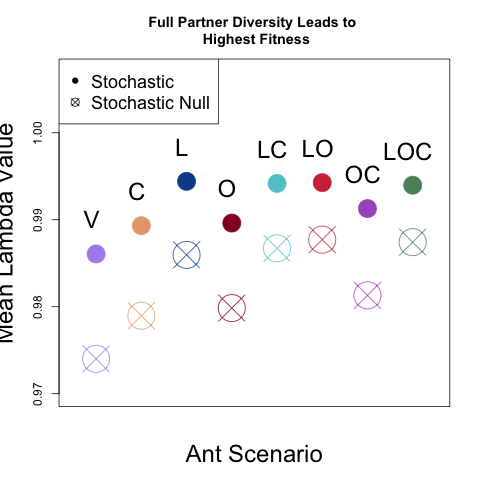
\includegraphics[width=0.95\linewidth]{Figures/LambdaMeans.png}
\end{figure}

%% Liom to all
%We are 100\%, 88\%, 90\%, and 76\% certain that having only \textit{L. apiculatum} ants as partners leads to a higher $\lambda$ than having no partners, only having \textit{C. opuntiae} ants as partners, only having other ants as partners, and having \textit{C. opuntiae} and other ants as partners respecitvely. 
%We are 96\%, 92\%, 92\%, and 84\% confident that having \textit{L. apiculatum} and \textit{C. opuntiae} ants as partners leads to a higher $\lambda$ than having no partners, only having \textit{C. opuntiae} ants as partners, only having other ants as partners, and having \textit{C. opuntiae} and other ants as partners respecitvely. 
%We are 98\%, 92\%, 96\%, and 92\% confident that having \textit{L. apiculatum} and other ants as partners leads to a higher $\lambda$ than having no partners, only having \textit{C. opuntiae} ants as partners, only having other ants as partners, and having \textit{C. opuntiae} and other ants as partners respecitvely. 
%We are 94\%, 84\%, 94\%, and 84\% confident that having only \textit{L. apiculatum}, \textit{C. opuntiae}, and other ants as partners leads to a higher $\lambda$ than having no partners, only having \textit{C. opuntiae} ants as partners, only having other ants as partners, and having \textit{C. opuntiae} and other ants as partners respecitvely. 
We are between 84\% and 100\% confident that any diversity scenario where \textit{L. apiculatum} ants are included as partners leads to a higher $\lambda$ for the tree cholla than any diversity scenario without these parnters.
These results indicate that sampling effect, not complementarity, is at play in this system.


%%%% Stochastic null follows similar patterns but dampened
Using the stochastic null IPM results, we found that when ant partners responded the same way to inter-annual variation similar patterns were found, though the magnitude of the patterns were somewhat different. 
We used the results of the stochastic null IPM to determine if portfolio effect is at play. 
We found that both the stochastic model and stochastic null model resulted in higher fitness when all ants are present compared to no partners 94\% of the time. 
These results differed in the magnitude of fitness boost recieved from partners.
In the stochastic IPM, tree cholla with all ants present resulted in a $\lambda$ that was 0.008 greater than tree cholla with no ants present; in the stochsatic null IPM, tree cholla with all ants rpesent resulted in a $\lambda$ that was 0.013 greater than tree cholla with no ants present. 
We are 52\% confidence that the difference is greater when inter-annual effects were not ant dependent (in the stochastic null model).
This indicates that portfolio effect is at play, if only weakly evident. 

\subsection*{Statistical Modeling}

\paragraph{Growth Model}
% Growth Model
\begin{figure}[H]
	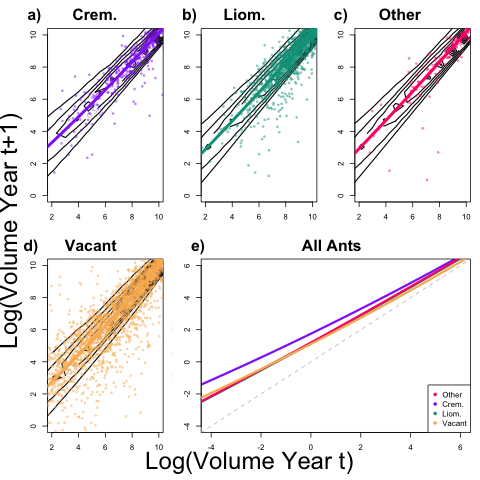
\includegraphics[width=0.95\linewidth]{Figures/GrowContourLinesColor.png}
	\caption{asdasdf}
	\label{fig:growth}
\end{figure}
Tree cholla experience positive mean growth rates across all partners at small to medium sizes with the highest chances of shrinking occurring at the largest sizes \ref{fig:growth}e.
The mean growth rate expected for plants that are 10 $cm^3$ or smaller in year t is 10.01 $cm^3/yr$, 4.65 $cm^3/yr$, 7.44 $cm^3/yr$, and 5.14 $cm^3/yr$ when tended by \textit{C. opuntiae}, \textit{L. apiculatum}, other ants, or no ants respectively. 
The mean growth rate expected for plants that are between 10 $cm^3$ and 150 $cm^3$ in year t is 2.81 $cm^3/yr$, 2.11 $cm^3/yr$, 2.49 $cm^3/yr$, and 1.75 $cm^3/yr$ when tended by \textit{C. opuntiae}, \textit{L. apiculatum}, other ants, or no ants respectively. 
The mean growth rate expected for plants that are larger than 150 $cm^3$ in year t is 1.28 $cm^3/yr$, 1.21 $cm^3/yr$, 1.29 $cm^3/yr$, and 1.10 $cm^3/yr$ when tended by \textit{C. opuntiae}, \textit{L. apiculatum}, other ants, or no ants respectively. 
Plants with \textit{C. opuntiae} ant partners experience the highest mean growth rates across all but the largest sizes, where they experience comprable growth to the other tended plants \ref{fig:growth}a. 
Plants with \textit{L. apiculatum} ants experience the lowest mean growth rates at the smallest sizes and the second lowest at all other sizes \ref{fig:growth}b. 
Plants with other ants experience the second highest mean growth rates across all but the largest sizes, were they experience the highest growth rates\ref{fig:growth}c.
Plants with no partners experience the second lowest growth rates at small sizes, after which they experience the lowest growth rates \ref{fig:growth}d. 


We are 89\%, 88\%, and 70\% confident that plants tended by \textit{C. opuntiae} ants experience higher mean growth rates across sizes than plants tended by no parnters, \textit{L. spiculatum} ants, or other ants respectively.
We are 89\%, 65\%, and 94\% confident that plants with no partners experience lower mean growth rates across all sizes than plants tended by \textit{C. opuntiae}, \textit{L. apiculatum}, or other ants respectively.

\paragraph{Survival Model}
% Survival Model
\begin{figure}[H]
	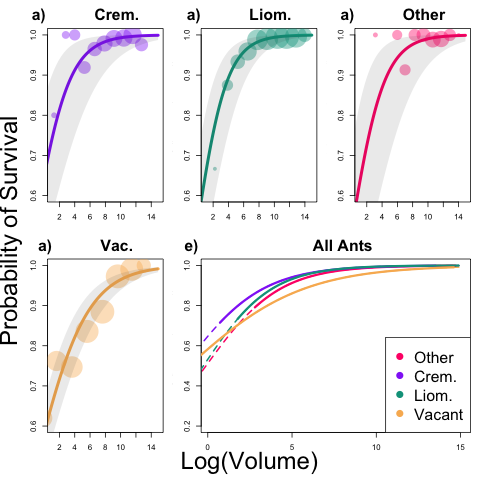
\includegraphics[width=0.95\linewidth]{Figures/SurvivalPlot.png}
	\caption{asdasdf}
	\label{fig:surv}
\end{figure}
Tree cholla experience between 7.7\% and 99.9\% survival rate depending on their size and ant partner \ref{fig:surv}e.
Smaller cacti all have lower survival rates, while larger cacti have higher survival rates, all nearing 100\% when they reach their largest observed sizes.
The mean survival rate expected for plants that are 10 $cm^3$ or smaller in year t is 48\%, 37\%, 37\%, and 47\% when tended by \textit{C. opuntiae}, \textit{L. apiculatum}, other ants, or no ants respectively. 
The mean survival rate expected for plants that are between 10 $cm^3$ and 150 $cm^3$ in year t is 90\%, 87\%, 84\%, and 80\% when tended by \textit{C. opuntiae}, \textit{L. apiculatum}, other ants, or no ants respectively. 
The mean survival rate expected for plants that are larger than 150 $cm^3$ in year t is 99\%, 99\%, 98\%, and 95\% when tended by \textit{C. opuntiae}, \textit{L. apiculatum}, other ants, or no ants respectively. 
Plants with \textit{C. opuntiae} ants experience the highest mean survival rates across all sizes \ref{fig:surv}a.
Plants with \textit{L. apiculatum} ants experience the lowest mean survival rates when small and the second highest mean survival rates across all other sizes \ref{fig:growth}b. 
Plants with other ants experience the second lowest mean survival rates across all sizes \ref{fig:growth}c.
Plants with no partners experience the second highest survival rates at small sizes, after which they experience the lowest survival rates \ref{fig:growth}d. 

We are 82\%, 63\%, and 100\% confident that plants tended by \textit{C. opuntiae} ants experience higher mean survival rates across all sizes than plants tended by no parnters, \textit{L. spiculatum} ants, or other ants respectively.
We are 82\%, 68\%, and 64\% confident that plants with no partners experience lower mean survival rates across all sizes than plants tended by \textit{C. opuntiae}, \textit{L. apiculatum}, or other ants respectively.

%% Flowers Model
\paragraph{Flowering Model}
There is a clear size effect on the number of flowers produced. 
The mean number of flowers produced by a plant remains at 0 until the plant reaches medium sizes after which the mean number of flower produced increases eponentially to about 40 flowers per plant per year at large sizes.
The mean number of flowers produced for a plant that is 150 $cm^3$ or smaller in year $t$ is <1 flower per plant.
The mean number of flowers produced for a plant that is larger than 150 $cm^3$ in year $t$ is 8.7 flowers per plant.


% Viability Model
\paragraph{Viability Model}
\begin{figure}[H]
	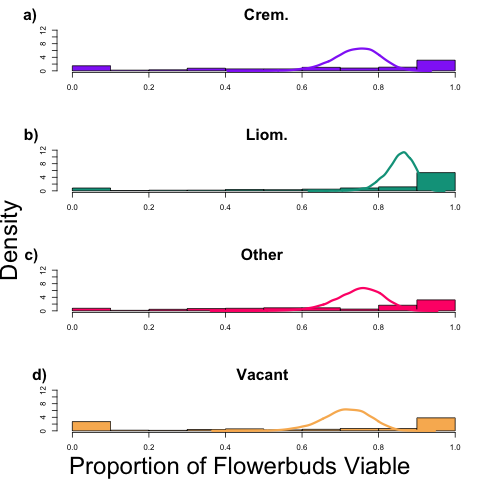
\includegraphics[width=0.95\linewidth]{Figures/ViabHist.png}
	\caption{asdasdf}
	\label{fig:viab}
\end{figure}
Tree cholla that are reproducing in year $t$ experience between 39\% and 96\% viability rates of flowers \ref{fig:viab}.
The ant partners make a difference in the mean viability rate of flowers, with \textit{L. apiculatum} tended plants experiencing the highest mean viability rate (at 86\%), followed by other tended plants (at 75\%), \textit{C. opuntiae} tended plants (at 74\%) and vacant plants (at 71\%).
We are 99\%, 98\%, and 97\% confident that \textit{L. apiculatum} tended plants experience higher viability rates than plants tended by no partners, \textit{C. opuntiae}, or other ants respectively.
We are 95\% and 69\% confident that vacant plants experience lower viability rates than plants tended by \textit{C. opuntiae} ants or other ants respectively.

%% Reproduction Model
\paragraph{Reproduction Model}
The probability of a plant reproducing in a given year is highly size dependent. 
The mean probability of reproducing remains at about 0\% until the plant reaches a medium size, after which the mean probability of reproducing increases steadily before reaching about 100\% at large sizes. 



%% Seeds Produced
\paragraph{Seeds Per Flower Model}
Each viable flower on a plant produces between 97 and 257 seeds.
This number is affected by the ant partner present. 
\textit{C. opuntiae} tended plants produce a mean of 148 seeds per flower. 
\textit{L. apiculatum} tended plants produce a mean of 149 seeds per flower. 
Vacant plants produce a mean of 160 seeds per flower. 
We are 73\% and 78\% confident that vacant plants produce more seeds per flower on average than plants tended by \textit{C. opuntiae} and \textit{L. apiculatum} ants respectively.


%% Precensus Survival\
\paragraph{Precensus Survival Model}
Pre-census seed survival rates fall between 0\% and 95\% with the mean pre-census seed survival at 18\%.

%% Germination
\paragraph{Germination Model}
Seeds have a significantly higher probability of germinating in year one than in year two.
Seeds in year one experience germination rates between 50\% and 100\% with a mean of 62\% germination.
Seeds in year two experience germination rates between 50\% and 98\% with a mean of 58\% germination.


%% Recruit size distribution
New recruits are expected to be between the sizes of 0.11 $cm^3$ and 0.38 $cm^3$ with a mean size of 0.20 $cm^3$.

%% Ant Transition Rates
\paragraph{Ant Transition Model}
\begin{figure}
	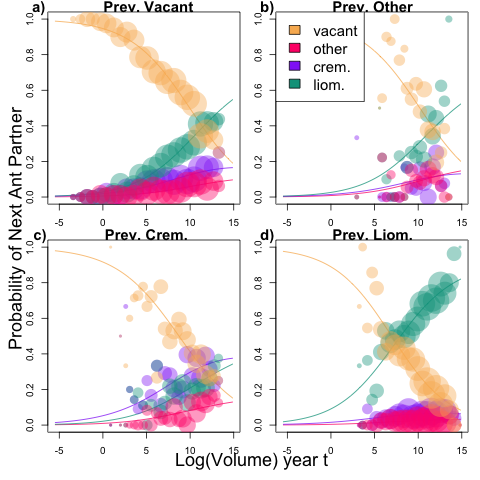
\includegraphics[width=0.95\linewidth]{Figures/AntSizeMulti.png}
\end{figure}
All small plants are most likely to be vacant, while large plants are much more likely to be occuplied by one ant or another. 
\textit{L. apiculatum} ants are the most likely tender in year $t+1$ for all large plants that were not previously tended by \textit{C. opuntiae} ants in year $t$, while \textit{C. opuntiae ants} tended plants in year $t$ are most likely to remain tended by \textit{C. opuntiae} ants in year $t+1$.
We are 93\%, 89\%, 86\%, and 93\% confident that plants that are smaller than 150 $cm^3$ in year $t$ will be vacant in year $t+1$ when they were tended by no partners, \textit{C. opuntiae}, \textit{L. apiculatum}, or other ants respectively in year $t$.

% Liom 
We are 75\%, 100\%, and 100\% confident that plants which were previously tended by \textit{L. apiculatum} and larger than 150 $cm^3$ in year $t$ are more likely to be tended by \textit{L. apiculatum} ants in year $t+1$ than be vacant, tended by \textit{C. opuntiae}, or other ants in year $t+1$.
We are 35\%, 100\%, and 100\% confident that plants which were previously vacant and larger than 150 $cm^3$ in year $t$ are more likely to be tended by \textit{L. apiculatum} ants in year $t+1$ than be vacant, tended by \textit{C. opuntiae}, or other ants in year $t+1$.
We are 32\%, 100\%, and 100\% confident that plants which were previously tended by other ants and larger than 150 $cm^3$ in year $t$ are more likely to be tended by \textit{L. apiculatum} ants in year $t+1$ than be vacant, tended by \textit{C. opuntiae}, or other ants in year $t+1$.

% Crem
We are 37\%, 100\%, and 100\% confident that plants which were previously tended by \textit{C. opuntiae} and larger than 150 $cm^3$ in year $t$ are more likely to be tended by \textit{C. opuntiae} ants in year $t+1$ than be vacant, tended by \textit{L. apiculatum}, or other ants in year $t+1$.

\ali{}{Or I can do this section like this:}
% Prev Vacant
Plants which were previously vacant will most likely remain vacant until large. 
We expect that between 81\% and 98\% of tree cholla which are smaller than 150 $cm^3$ with no partners in year $t$ are going to be vacant in year $t+1$.
We expect that between 11\% and 55\% of tree cholla which are larger than 150 $cm^3$ with no partners in year $t$ are going to be tended by \textit{L. apiculatum} ants in year $t+1$.
We expect that between 6\% and 17\% of tree cholla which are larger than 150 $cm^3$ with no partners in year $t$ are going to be tended by \textit{C. opuntiae} ants in year $t+1$.
We expect that between 2\% and 10\% of tree cholla which are larger than 150 $cm^3$ with no partners in year $t$ are going to be tended by other ants in year $t+1$.

% Prev Crem
Plants which were previously tended by \textit{C. opuntiae} will most likely be vacant or tended by \textit{C. opuntiae} ants in the next year depending on size. 
We expect that between 74\% and 97\% of tree cholla which are smaller than 150 $cm^3$ and tended by \textit{C. opuntiae} in year $t$ are going to be vacant in year $t+1$.
We expect that between 8\% and 34\% of tree cholla which are larger than 150 $cm^3$ and tended by \textit{C. opuntiae} in year $t$ are going to be tended by \textit{L. apiculatum} ants in year $t+1$.
We expect that between 15\% and 38\% of tree cholla which are larger than 150 $cm^3$ and tended by \textit{C. opuntiae} in year $t$ are going to be tended by \textit{C. opuntiae} ants in year $t+1$.
We expect that between 3\% and 13\% of tree cholla which are larger than 150 $cm^3$ and tended by \textit{C. opuntiae} in year $t$ are going to be tended by other ants in year $t+1$.

% Prev Liom
Plants which were previously tended by \textit{L. apiculatum} will most likely be vacant or tended by \textit{L. apiculatum} in the next year depending on size. 
We expect that between 64\% and 97\% of tree cholla which are smaller than 150 $cm^3$ and tended by \textit{L. apiculatum} in year $t$ are going to be vacant in year $t+1$.
We expect that between 30\% and 82\% of tree cholla which are larger than 150 $cm^3$ and tended by \textit{L. apiculatum} in year $t$ are going to be tended by \textit{L. apiculatum} ants in year $t+1$.
We expect that between 4\% and 7\% of tree cholla which are larger than 150 $cm^3$ and tended by \textit{L. apiculatum} in year $t$ are going to be tended by \textit{C. opuntiae} ants in year $t+1$.
We expect that between 1\% and 3\% of tree cholla which are larger than 150 $cm^3$ and tended by \textit{L. apiculatum} in year $t$ are going to be tended by other ants in year $t+1$.

% Prev Other
Plants which were previously tended by other ants will most likely be vacant or tended by other ants in the next year depending on size. 
We expect that between 82\% and 99\% of tree cholla which are smaller than 150 $cm^3$ and tended byother ants in year $t$ are going to be vacant in year $t+1$.
We expect that between 10\% and 53\% of tree cholla which are larger than 150 $cm^3$ and tended by other ants in year $t$ are going to be tended by \textit{L. apiculatum} ants in year $t+1$.
We expect that between 4\% and 13\% of tree cholla which are larger than 150 $cm^3$ and tended by other ants in year $t$ are going to be tended by \textit{C. opuntiae} ants in year $t+1$.
We expect that between 3\% and 15\% of tree cholla which are larger than 150 $cm^3$ and tended by other ants in year $t$ are going to be tended by other ants in year $t+1$.


\section*{Discussion}
The large, long-lived tree cholla produce EFN which tempts several species of ant partners to protect them from herbivores and seed predators. 
Many studies have looked at multispecies mutualisms and the how having a variety of partners leads to variation in demographic effects \cite{Palmer2010, Bascompte2019, Stachowicz2005, Ford2015, Baez2016}. 
Because these tree cholla interact with only one ant partner at a time, it is a unique system in which to parse out the individual effects of each ant partners, both in isolated settings or in combinations we cannot test in the real world.


%\subsection*{Demographic effects of association with alternative partners}
We asked what effects the partners which interact with tree cholla (\textit{C. opuntiae},\textit{L. apiculatum}, and more) have on the vital rates of tree cholla. 
Using a system of heirarchical bayesian models we found that there were discernable differences in the effects that each partner had on vital processes of the focal mutualist. 
The different vital rates vary in importance across tree cholla ontogeny.
Several of them are negatively impacted by the presence and pressure of herbivores and seed predators \cite{Miller2009, Miller2006} and positively impacted by the presence of ant partners \cite{Miller2007}.
The predators and herbivores target new growth and flowers, leading to negative impacts on the growth rates, survival rates, and floral viability rates of tree cholla \cite{Louda1995, Agrawal2004}.
The presence of the ant partners can reduce those negative effects.


It has been previously hypothesized that their is a heirarchy of partners due to the ability for \textit{L. apiculatum} ants to defend the cacti from seed predators and herbivores \cite{Miller2007}.
These prior results would suggest that all vital rates that are affected by ant partners would be boosted the most by the presence of \textit{L. apiculatum} ants, this is not what we found. 
Our results suggest that different partners differ significantly in their effects on vital rates.

Prior to reproduction, the tree cholla experience only growth and survival.
\textit{C. opuntiae} tended ants are associated with the highest growth rates and survival rates of plants. 
This indicates that \textit{C. opuntiae} ants may be good ants for pre-reproductive tree cholla plants. 
Reproducing plants experience a probability of reproducing, flower production, and floral abortion.
Floral abortion is heavily affected by seed predators \cite{Miller2008}, which the ants defend the cacti, leading to increased floral viability.
We specifically found that tree cholla experienced the highest floral viability rates when tended by \textit{L. apiculatum} ants. 
This indicates that \textit{L. apiculatum} ants may be good partners for reproducing plants. 

These results together would suggest that complementarity may be the underlying mechanism that explains why partner diversity is beneficial in this system. 


%\subsection*{Frequency and direction of partner turnover}
We have shown that the identity of partners is important to the processes that define tree cholla fitness. 
Now we need to analyze the dynamics of partner turnover which dictate the identity of tree cholla partners and therefore the effects of vital rates on the tree cholla. 
With our models we were able to identify both the direction, frequency, and distinct patterns of partner turnover. 

In the literature, it is clear that the frequency of partner turnover can have big effects on the fitness of the focal mutualist \cite{Fiala1994, Horvitz1986, Oliveira1999, Sachs2004}.
In some systems high freqency of turnover is necessary to resiliency and leads to higher fitness benefits \cite{Trojelsgaard2015}, while in other systems loyalty is the most beneficial \cite{Batstone2018}.
While the purpose of this paper is not to establish which would be most beneficial in this system, we were able to identify the pattern. 
Small plants are almost entirely vacant in this system until they grow large enough to begin producing significant amounts of EFN.
Our model shows that once they do produce EFN, plants experience a relatively significant amount of turnover.
Mid-sized and large plants which were either vacant or tended by other ants are most likely to become tended by \textit{L. apiculatum} ants in the next year, thereby experiencing partner turnover. 
Plants which were tended by \textit{L. apiculatum} or \textit{C. opuntiae} ants are most likely to remain tended by the same partners multiple years in a row. 
This indicates that \textit{C. opuntiae} ants and \textit{L. apiculatum} ants are loyal partners which retain the same plants year after year with regularity.


As established in previous studies, the direction of partner turnover is important when the identity of partners impacts the quality of benefits recieved \cite{Fonseca2003, Alonso1998, Dejean2008, Noe1994}.
In our study we found that there are distinct patterns to the direction of partner turnover. 
Specifically, most plants are tended by \textit{L. apiculatum} ants at some point, because vacant plants, other tended plants, and \textit{L. apiculatum} tended plants are all most likely to be tended by \textit{L. apiculatum} ants.
This indicates that while \textit{L. apiculatum} ants are loyal to their own plants and return multiple years in a row to the same ones, they are also strong colonizers. 


%\subsection*{Effect of partner diversity on plant fitness and what mechanisms explain this}
The combination of partner identity, partner turnover, and temporal stochasticity gives us the unique power to consider both the fitness of the tree cholla under different partner scenarios (as some have done before \cite{Palmer2010}) and a unique set of mechanisms (\cite{Batstone2018}) which explain how the multi-partner interactions lead to fitness differences. 
We found that the combination of accurate partner transitions with partner identity affected the fitness of the tree cholla in interesting and dynamic ways. 
Namely, a best partner emerged in this analysis, which was surprising given the nature of our vital rate findings. 
The variation in best partner for each vital rate suggested the potential that the different ant partners had some level of unique specialty in what they offered, which would support complementarity as the mechanism which explained the effects of partner diveristy \cite{Stachowicz2005, Stanton2003}. 
The results of our IPM however differ from this prediction. 

Using the stochastic IPM we developed, we found evidence of sampling effect rather than complementarity.
We found that \textit{L. apiculatum} was the single best partner, and that all diversity scenarios where \textit{L. apiculatum} was present resulted in the highest possible fitness of tree cholla. 
This indicates that despite the fact that \textit{L. apiculatum} partnership does not result in the highest growth and survival rates, it is still the overall best partner. 

Using the stochastic null IPM and the stochastic IPM we compared the fitness boost recieved by all ant partners when ants effects varied separately across years and when they did not. 
When all ants responded to inter-annual variability the same way (shown in the stochastic null IPM) we found that the fitness boost recieved from partners was larger than the fitness boost recieved when ants responded to inter-annual variability differently.
This indicates that having multiple possible partners benefits the tree cholla by buffering the potentially negative effects of inter-annual variation. 

%\subsection*{Synthesis????? All together}
\ali{}{What this all means more broadly?? I'm currently not sure what to do with this}
This paper shows the importance of long-term datasets in investigating species interactions and calls for further use of long-term data. 
Previously studies have analyzed how partner identity and partner turnover impact focal mutualist fitness \cite{Fonseca2003, Dejean2008, Noe1994, Barrett2015, Bruna2014, Trojelsgaard2015}.
Separate studies have analyzed how inter-annual variability impacts focal mutualists \cite{Alonso1998, Alarcon2008, Ollerton2006, Horvitz1990, Lazaro2022}.
The long term dataset we used gave us the unique ability to consider the combined effects of partner identity, partner turnover, and temporal stochasticity.


%\subsection*{Future Directions}
This paper has limitations, specifically surrounding the driving forces behind the ant-plant interactions.
We revealed the dynamics of partner turnover and showed that different ant partners are correlated with different fitness benefits.
As of now, the driving mechanisms behind how ant species come to interact with individual plants is still unknown and could be subject to future work. 


\section*{Acknowledgments}

%%%%%%%%%%%%%%%%%%%%%
% Statement of Authorship
%%%%%%%%%%%%%%%%%%%%%
% This section should also be commented out while your MS is undergoing
% double-blind review. The specifics should of course be adapted to
% your paper, but the paragraph below gives some hints of possible
% contributions.

\section*{Data and Code Availability}

\section*{Appendix A: Additional Methods and Parameters}

% In most cases, authors should typeset supplementary material in a separate,
% author-supplied PDF. For author-supplied PDFs, please consult the
% AmNat_supp_template.tex document, available from
% https://www.journals.uchicago.edu/journals/an/instruct 
%
% By contrast, the Appendix instructions below apply to cases in which
% a brief appendix is to appear in print after the main body of the article.
% That notably includes descriptions of methods, tables defining parameters,
% and other material necessary for reproducing the MS's results.
%
% Please reset counters for the appendix (thus normally figure A1, 
% figure A2, table A1, etc.).
%
% Most AmNat articles have no more than one print appendix. If your article
% has more than one, counters for each appendix should match the letter of
% that appendix. For example, tables in Appendix B should be numbered table B1, % table C2, etc. This applies to tables, equations, and figures.
%
% It's better not to use the \appendix command, because we have some
% formatting peculiarities that \appendix conflicts with.

\renewcommand{\theequation}{A\arabic{equation}}
% redefine the command that creates the equation number.
\renewcommand{\thetable}{A\arabic{table}}
\setcounter{equation}{0}  % reset counter 
\setcounter{figure}{0}
\setcounter{table}{0}

%%%%%%%%%%%%%%%%%%%%%
% Bibliography
%%%%%%%%%%%%%%%%%%%%%
% You can either type your references following the examples below, or
% compile your BiBTeX database and paste the contents of your .bbl file
% here. The amnatnat.bst style file should work for this---but please
% let us know if you run into any hitches with it!
%
% If you upload a .bib file with your submission, please upload the .bbl
% file as well; this will be required for typesetting.
%
% The list below includes sample journal articles, book chapters, and
% Dryad references.
\bibliographystyle{apalike}
\bibliography{References.bib}


\newpage{}

\section*{Tables}
\renewcommand{\thetable}{\arabic{table}}
\setcounter{table}{0}

\renewcommand{\thetable}{\arabic{table}}
\setcounter{table}{0}

% I am creating a table here to include all parameter estimations and descriptions
  \begin{table}[]
  \begin{tabular}{l|l|l}
    \textbf{Parameter} & \textbf{Median ($95\%$ CI)} & \textbf{Prior Distribution} \\
    \hline
    %% Growth Parameters
    growth xi intercept vacant $\beta_{01}^g$ & $-5.210899 (-5.686865, -5.491787)$ & sDE\\
    growth xi intercept other $\beta_{02}^g$ & $-5.8288 (-5.956217, 1.766021) $&asdf \\
    growth xi intercept \textit{C. opuntiae} $\beta_{03}^g$ & $-4.529523 (-6.0770390, 0.1222112)$ & asdf\\
    growth xi intercept \textit{L. apiculatum} $\beta_{04}^g$ & $-5.106802 (-5.4499944, 0.5453901)$ & asdf\\
    growth xi size dependent vacant $\beta_{11}^g$ & asdf&asdf \\
    growth xi size dependent other $\beta_{12}^g$ & asdf&asdf \\
    growth xi size dependent \textit{C. opuntiae} $\beta_{13}^g$ & asdf&asdf \\
    growth xi size dependent \textit{L. apiculatum} $\beta_{14}^g$ &sadf &asdf \\
    growth omega intercept $\omega_0^g$ & & \\
    growth omega size dependent $\omega_1^g$ & & \\
    growth alpha intercept $\alpha_0^g$ & & \\
    growth alpha size dependent $\alpha_1^g$ & & \\
    \hline
    %% Germination Parameters
    1-year germination intercept $\alpha^{\gamma_1}$ & & \\
    2-year germination intercept $\alpha^{\gamma_2}$ & & \\
    \hline
    %% Survival Parameters
    survival intercept vacant $\beta_{01}^s$ & & \\
    survival intercept other $\beta_{02}^s$ & & \\
    survival intercept \textit{C.opuntiae} $\beta_{03}^s$ & & \\
    survival intercept \textit{L. apiculatum} $\beta_{04}^s$ & & \\
    survival size dependent vacant $\beta_{11}^s$ & & \\
    survival size dependent other $\beta_{12}^s$ & & \\
    survival size dependent \textit{C. opuntiae} $\beta_{13}^s$ & & \\
    survival size dependent \textit{L. apiculatum} $\beta_{14}^s$ & & \\
    \hline
    %% Probability of Flowering Parameters
    flowering intercept $\beta_0^f$ & & \\
    flowering size dependent $\beta_1^f$ & & \\
    \hline
    %% Floral Viability Parameters
    viability intercept vacant $\beta_01^v$ & & \\
    viability intercept other $\beta02^v$ & & \\
    viability intercept \textit{C. opuntiae} $\beta_03^v$ & & \\
    viability intercept \textit{L. apiculatum} $\beta_04^v$ & & 
  \end{tabular}
  \end{table}

\section*{Figure legends}


%%%%%%%%%%%%%%%%%%%%
 Videos
%%%%%%%%%%%%%%%%%%%%
 If you have videos, journal style for them is generally similar to that for
 figures. 

%%%% Include the text below if you have videos



%%%% Include the above if you have videos


\end{document}
